\documentclass[aip,jcp,reprint,longbibliography,floatfix]{revtex4-2}

\usepackage{graphicx}
\usepackage{amsmath,amssymb,mathtools,bm}
\usepackage{booktabs}
\usepackage{placeins}
\usepackage{siunitx}
\usepackage{verbatim}
\usepackage{array}
\usepackage{xcolor}
\usepackage{tikz}
\usetikzlibrary{arrows.meta,backgrounds,fit,positioning}
\definecolor{FrameworkBlue}{HTML}{245C73}
\definecolor{FrameworkTeal}{HTML}{2F8F83}
\definecolor{FrameworkGold}{HTML}{C88A2D}
\definecolor{FrameworkSlate}{HTML}{4A5561}
\definecolor{FrameworkInk}{HTML}{263238}
\emergencystretch=2em

\begin{document}

\title{Algorithmic Construction and Exploitation of Topology-Constrained Refinement Models for Semiexperimental Equilibrium Structures}

\author{Vincenzo Barone}
\email{vincebarone52@gmail.com}
\affiliation{INSTM, National Interuniversity Consortium for Materials Science and Technology, via G. Giusti 9, 50121 Firenze, Italy}

\begin{abstract}

Semiexperimental equilibrium structures combine high-resolution rotational spectroscopy with computed vibrational and electronic corrections. The numerical solution of a least-squares refinement is now routine; the chemically decisive step is often the earlier one, namely the construction and validation of the inverse model that connects precise observables with structural parameters. Active coordinates, symmetry, weakly determined directions, constraints, predicates, and parameter classes are still frequently selected by expert intervention, especially for cyclic, fused, and bridged molecular graphs.

This paper introduces \texttt{MORPHEUS} (Model Optimization and Refinement from Perceived Hierarchy, Equivalence, Uncertainty, and Symmetry), a framework that turns model formulation into a reproducible, auditable construction step constrained by symmetry and rank. The semiexperimental refinements reported here provide the principal validation, but the construction is more general: it builds constrained refinement models from topology, symmetry, rank, isotope coverage, and external reference information before any numerical least-squares solution is attempted. Molecular topology defines the primitive coordinate space, symmetry selects the admissible active subspace, isotopic coverage determines which directions are experimentally supported, and electronic-structure reference information enters only through explicit primitive-coordinate constraints, predicates, or parameter classes.

Within MATRIX, ORACLE supplies topology, point-group operations, continuous
equivalence descriptors and the redundant primitive/Wilson-B source. SMITH
constructs the corresponding SONIC coordinate contract, and MORPHEUS
formulates and solves the inverse model without repeating either molecular
perception or coordinate construction.

Two equivalent active spaces are available: symmetry-adapted generalized internal coordinates built from homogeneous primitive families, and symmetry-adapted Cartesian displacements after removal of translations and rotations. The chemical interface remains internal-coordinate based, so bond, angle, dihedral, out-of-plane, ring, and local-frame relations have the same meaning whichever numerical basis is used. Validation on acyclic, cyclic, planar, fused, bridged, and flexible systems shows that rank, effective dimension, residuals, structural parameters, and propagated uncertainties are reproduced without manual coordinate-model formulation. In the norbornane-derived series, norcamphor probes a bridged reduced-dimensionality model and camphor adds methyl substitution as a stricter validation test: the accepted no-Kraitchman BDPCS3-predicate model gives sub-milliangstrom bond corrections, whereas superficially competitive variants based on unsupported hydrogen directions or tight Kraitchman predicates are rejected because they distort the geometry. The testosterone case study then shows that accurate quantum chemical equilibrium geometries, accelerated vibrational corrections, and generated topology-constrained refinement models can be chained for molecular systems containing about 50 atoms, where isotope-rich data sets required by conventional refinement strategies are generally unavailable.

\end{abstract}

\keywords{semiexperimental equilibrium structures, model validation, generalized internal coordinates, topology-constrained refinement, Kraitchman equations}

\maketitle


\section{Introduction}

Accurate equilibrium molecular structures are central to rotational
spectroscopy, thermochemistry, force-field development, and the validation of
electronic-structure methods.\cite{Demaison2011EquilibriumStructures,PuzzariniStanton2023}
Despite decades of progress in semiexperimental refinement, model construction
remains largely a manual activity. Structure determination from experimental
observables is a coordinate-dependent inverse problem: the data constrain a
Cartesian geometry, but the fitted variables determine conditioning,
constraints, correlations, and uncertainties. Rotational spectroscopy is a
stringent example because rotational constants probe the molecular mass
distribution with high precision, whereas semiexperimental
($r_e^{\mathrm{SE}}$) structures require vibrational and sometimes electronic
corrections to convert ground-state constants into equilibrium
information.\cite{Costain1958,Pawlowski2002,Piccardo2015B3LYP,Penocchio2015B2PLYP}

Modern fitting programs and workflows\cite{Mendolicchio2017MSR,KisielPROSPE,Kanzow2025PCCP}
have established robust statistical principles: fit well-conditioned
observables, include theoretical predicates when experimental information is
incomplete, and propagate covariance to derived structural
parameters.\cite{Bartell1975Predicate} Their common prerequisite is that the
refinement model has already been formulated. This prerequisite is especially
restrictive for rings, fused systems, and bridged frameworks, where equivalent
paths through the molecular graph can make one internal coordinate primary and
another derived. The target of the present work is therefore not a new
least-squares observable or a molecule-specific improvement in residuals, but
an algorithmic route from molecular topology to a reproducible statistical
refinement model.

In this implementation, the non-redundant internal-coordinate family is
\texttt{SONIC} (Symmetry-Oriented Non-redundant Internal Coordinates), and
\texttt{SMITH} is the standalone builder that constructs the corresponding
coordinate contracts. ORACLE provides the redundant primitive coordinates and
their analytic Wilson $\mathbf{B}$ rows; SMITH transforms this source into the
non-redundant, symmetry-adapted GIC basis and symmetry-adapted Cartesian
reference spaces, with symmetry labels and provenance. \texttt{MORPHEUS} is the refinement layer built on those
frozen definitions: it selects experimentally supported directions, applies
constraints, classes, and predicates, solves the least-squares problem, and
tests the stability of the accepted model. The molecular-state perception is
supplied by \texttt{ORACLE}, which develops the continuous molecular perception
and synthon descriptors introduced in earlier work.\cite{Lazzari2020Proxima,Lazzari2024SynthonPCS}
The current contract keeps the continuous topological edge order distinct from
the Mayer/Pauling multiplicity and resolves the latter into $\sigma$,
first-$\pi$ and second-$\pi$ ($\pi\pi$) indices; the latter two are retained
as separate synthon-similarity axes rather than collapsed into one
multiple-bond label.
Thus topology, symmetry operations, chemical descriptors, coordinate
definitions, and derivative conventions are fixed once; \texttt{MORPHEUS} uses
that contract without regenerating the model during refinement.
The parameter classes introduced below are statistical equality or predicate
relations for the semiexperimental inverse problem. They are not ZION atom
classes or force-field parameters: construction and evaluation of ZION remain
the separate responsibility of ARCHITECT, and are not required by MORPHEUS.

Recent workflows have extended semiexperimental refinement by combining
computed starting geometries, quantum chemical (QC) vibrational corrections, and
reduced-dimensionality models.\cite{Mendolicchio2025FastDvib} The implementation
developed here uses such data as upstream inputs while making the refinement
model itself derived from the molecular graph rather than hand specified.
Reference geometries from QC computations or from fragment libraries (e.g.,
LCB25\cite{Lazzari2025LCB25}) enter only as chemically explicit constraints,
predicates, or parameter classes; the fitted variables remain the
non-redundant active coordinates generated from topology. The framework
therefore converts accurate QC structures and vibrational corrections into an
explicit, rank-audited refinement model without molecule-specific coordinate
design.

The procedure starts from Cartesian coordinates. Primitive general internal
coordinates (GICs) are generated from perceived topology, symmetry is assigned,
and the totally symmetric active space is defined. Isotope coverage, symmetry
orbits, chemical descriptors, and reference data then generate compatible
constraints, predicates, and parameter classes. Two active spaces are available:
symmetry-adapted GICs and symmetry-adapted Cartesians after removal of
translations and rotations. Constraints remain primitive internal-coordinate
relations and are projected onto either active basis by the Wilson matrix or the
corresponding derivative operator.\cite{Wilson1955}

The rotational semiexperimental problem is used here as a demanding test
because it exposes both rank deficiencies and chemically meaningful
constraints. The validation set is organized so that each system probes a
different failure mode of manual model formulation: acyclic references, ring
closures, planar-component selection, fused and bridged topology, homologous
series with different isotopic coverage, reduced-dimensionality constraints,
and finally a large-molecule scale demonstration.


\section{Theory and Method}

\subsection{Overview of the Framework}

The overall architecture is summarized in
Figure~\ref{fig:workflow-architecture}. The key separation is between the
chemical model, the numerical active basis, and the least-squares solution.
Chemical information is always expressed in primitive internal coordinates;
the active variables may be GIC amplitudes or symmetry-adapted Cartesian
displacements. This separation is what makes the generated model traceable:
the same primitive relation has the same chemical meaning regardless of the
basis used to solve the refinement.

\begin{figure*}
\centering
\resizebox{0.92\textwidth}{!}{%
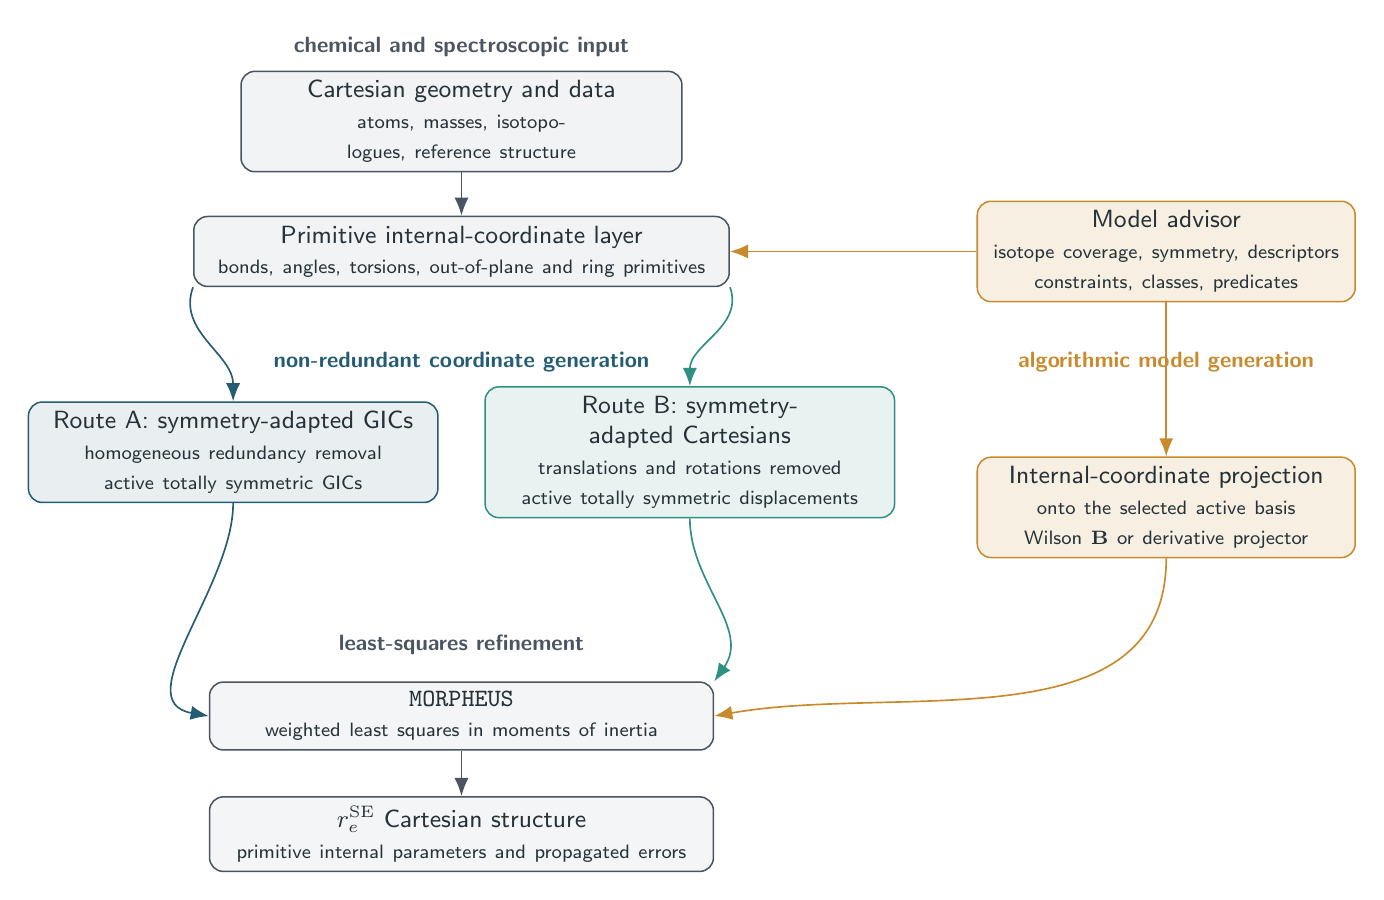
\begin{tikzpicture}[
  x=1cm,
  y=1cm,
  font=\sffamily\small,
  box/.style={
    draw,
    rounded corners=5pt,
    align=center,
    minimum height=0.82cm,
    line width=0.55pt,
    text=FrameworkInk,
    fill=white
  },
  inputbox/.style={box, fill=FrameworkSlate!7, draw=FrameworkSlate, minimum width=5.6cm, text width=5.2cm},
  primbox/.style={box, fill=FrameworkSlate!7, draw=FrameworkSlate, minimum width=6.8cm, text width=6.4cm},
  gicbox/.style={box, fill=FrameworkBlue!10, draw=FrameworkBlue, minimum width=5.2cm, text width=4.9cm},
  cartbox/.style={box, fill=FrameworkTeal!11, draw=FrameworkTeal, minimum width=5.2cm, text width=4.9cm},
  sidebox/.style={box, fill=FrameworkGold!14, draw=FrameworkGold, minimum width=4.8cm, text width=4.4cm},
  outbox/.style={box, fill=FrameworkSlate!6, draw=FrameworkSlate, minimum width=6.4cm, text width=6.0cm},
  arrow/.style={-{Latex[length=2.3mm,width=1.8mm]}, line width=0.60pt, draw=FrameworkSlate},
  gicarrow/.style={arrow, draw=FrameworkBlue},
  cartarrow/.style={arrow, draw=FrameworkTeal},
  sidearrow/.style={arrow, draw=FrameworkGold}
]
\node[font=\footnotesize\bfseries\sffamily, text=FrameworkSlate] at (-3.4,0.95) {chemical and spectroscopic input};
\node[font=\footnotesize\bfseries\sffamily, text=FrameworkBlue] at (-3.4,-3.05) {non-redundant coordinate generation};
\node[font=\footnotesize\bfseries\sffamily, text=FrameworkGold] at (5.55,-3.05) {algorithmic model generation};
\node[font=\footnotesize\bfseries\sffamily, text=FrameworkSlate] at (-3.4,-6.65) {least-squares refinement};

\node[inputbox] (geom) at (-3.4,0) {Cartesian geometry and data\\{\scriptsize atoms, masses, isotopologues, reference structure}};
\node[primbox] (prim) at (-3.4,-1.65) {Primitive internal-coordinate layer\\{\scriptsize bonds, angles, torsions, out-of-plane and ring primitives}};
\node[sidebox] (relations) at (5.55,-1.65) {Model advisor\\{\scriptsize isotope coverage, symmetry, descriptors}\\{\scriptsize constraints, classes, predicates}};

\node[gicbox] (gicroute) at (-6.3,-4.20) {Route A: symmetry-adapted GICs\\{\scriptsize homogeneous redundancy removal}\\{\scriptsize active totally symmetric GICs}};
\node[cartbox] (cartroute) at (-0.5,-4.20) {Route B: symmetry-adapted Cartesians\\{\scriptsize translations and rotations removed}\\{\scriptsize active totally symmetric displacements}};
\node[sidebox] (project) at (5.55,-4.90) {Internal-coordinate projection\\{\scriptsize onto the selected active basis}\\{\scriptsize Wilson $\mathbf{B}$ or derivative projector}};
\node[outbox] (sefit) at (-3.4,-7.55) {\texttt{MORPHEUS}\\{\scriptsize weighted least squares in moments of inertia}};
\node[outbox] (result) at (-3.4,-9.05) {$r_e^{\mathrm{SE}}$ Cartesian structure\\{\scriptsize primitive internal parameters and propagated errors}};

\draw[arrow] (geom) -- (prim);
\draw[sidearrow] (relations.west) -- (prim.east);
\draw[gicarrow] (prim.south west) to[out=-110,in=90] (gicroute.north);
\draw[cartarrow] (prim.south east) to[out=-70,in=90] (cartroute.north);
\draw[sidearrow] (relations.south) -- (project.north);
\draw[gicarrow] (gicroute.south) to[out=-90,in=170] (sefit.west);
\draw[cartarrow] (cartroute.south) to[out=-90,in=55] (sefit.north east);
\draw[sidearrow] (project.south) to[out=-90,in=10] (sefit.east);
\draw[arrow] (sefit) -- (result);
\end{tikzpicture}
}
\caption{Architecture of the model-generation framework.}
\label{fig:workflow-architecture}
\end{figure*}


\subsection{Primitive and Work Coordinates}

The coordinate construction starts from Cartesian geometry and perceived
topology. ORACLE uses bonded pairs and ring connectivity to define the
redundant primitive internal-coordinate (PIC) set and its Wilson matrix. The
PIC set contains
coordinates:  stretches, valence angles, torsions, out-of-plane deformations,
linear bends, and ring-specific primitives. Redundancy is intentional at this
stage because it lets topology, not a manually chosen reference path, decide
which combinations survive. For cyclic systems, endocyclic valence-angle
combinations describe ring bending, whereas \(n-3\) cyclic Fourier
combinations of native signed out-of-plane sources define the ring-puckering
rows. For the ordered stencil \(D(a,b,c,d)\), the native source is
\(U(b,a,d,c)\); the dihedral fixes only the cyclic ordering. Global
Cremer--Pople-like descriptors such as $q$ and $\phi$ are derived from these
rows. The local U construction is their closest curvilinear analogue, not an
identification with the global amplitudes and phases.  For each cosine--sine
pair, \(q_m=[(RPck_m^c)^2+(RPck_m^s)^2]^{1/2}\) and
\(\phi_m=\operatorname{atan2}(RPck_m^s,RPck_m^c)\), so
monocyclic, fused-ring, bridged, and polycyclic systems are handled by the
same machinery.\cite{CremerPople1975} This
primitive layer is also the chemical interface for constraints, predicates,
and parameter classes.


\subsection{Coordinates for Parameter Refinement}

The active space must be non-redundant, symmetry-consistent, and compatible
with chemically meaningful constraints. In the GIC route, topological
primitives are reduced within homogeneous families, so stretches, bends,
torsions, out-of-plane motions, and ring coordinates cannot replace one
another during rank reduction.\cite{PulayFogarasi1992,Peng1996Redundant,Baker1996Delocalized,BakkenHelgaker2002,Marenich2025GIC}
ORACLE generates the local primitive families and evaluates their Wilson
$\mathbf{B}$ matrix. SMITH consumes that frozen source, removes within-family
redundancies, forms the symmetry-adapted combinations, and stores the
transformed rows as \texttt{SONIC} coordinate contracts. They are documented in
the companion SMITH/SONIC methodological manuscript;
the present paper uses the resulting coordinate and derivative objects only as
the fixed input to the refinement-model layer. This boundary is deliberate: the
present work examines how generated coordinate spaces are coupled to isotopic
coverage, rank, constraints, predicates, parameter classes, and validation
diagnostics.
In the Cartesian route, translations and rotations are removed from the
Cartesian displacement space. In both cases symmetry selects the totally
symmetric active block and completes primitive constraints over equivalent
orbits.

At a reference geometry $\mathbf{x}_0$, primitive ($\Delta s$) and Cartesian
($\Delta x$) displacements are related to first order by the Wilson matrix\cite{Wilson1955}

\begin{equation}
\Delta \mathbf{s}
=
\mathbf{B}_s
\Delta \mathbf{x},
\qquad
\mathbf{B}_s =
\left.
\frac{\partial \mathbf{s}}
{\partial \mathbf{x}}
\right|_{\mathbf{x}_0}.
\end{equation}

For each homogeneous primitive family $\alpha$, the Wilson block
$\mathbf{B}_{s_\alpha}$ is submitted to a singular-value
decomposition (SVD),\cite{GolubReinsch1970}

\begin{equation}
\mathbf{B}_{s_\alpha}
=
\frac{\partial\mathbf{s}_\alpha}
{\partial\mathbf{x}} .
\end{equation}

\begin{equation}
\mathbf{B}_{s_\alpha}
=
\mathbf{U}_{\alpha}
\boldsymbol{\Sigma}_{\alpha}
\mathbf{V}_{\alpha}^{T},
\end{equation}

The retained left-singular vectors define the row-orthonormal transformation

\begin{equation}
\mathbf{R}_{\alpha}
=
\mathbf{U}_{\alpha,r}^{T},
\end{equation}

where the subscript $r$ denotes the retained singular subspace. The
non-redundant coordinates for family $\alpha$ are then

\begin{equation}
\Delta \mathbf{q}_\alpha
=
\mathbf{R}_\alpha
\Delta \mathbf{s}_\alpha ,
\qquad
\mathbf{B}_{q_\alpha}
=
\mathbf{R}_\alpha
\mathbf{B}_{s_\alpha}.
\end{equation}

The retained rank in each family gives the number of coordinates in that
family. Stacking the blocks gives

\begin{equation}
\Delta \mathbf{q}
=
\mathbf{R}
\Delta \mathbf{s},
\qquad
\mathbf{B}_{q}
=
\mathbf{R}
\mathbf{B}_s .
\end{equation}

The block-diagonal structure preserves chemical homogeneity. A stretch can
therefore not remove a torsion from the model, and a ring coordinate cannot be
lost because a different primitive family happened to enter the rank test
first. After family-wise reduction, residual dependencies are pruned with
deterministic topological tie breaking and the final basis is checked against
the expected vibrational rank.
This is a restriction on the admissible coordinate transformations, not on the
rank test itself. A global SVD of the full redundant primitive set would also
produce an orthonormal basis for the row space, but its left singular vectors
are free to mix primitives with different chemical meaning whenever their
Cartesian derivatives are linearly coupled or nearly degenerate. The numerical
rank would be correct, whereas the resulting coordinates could contain
arbitrary stretch--bend--torsion admixtures whose composition changes with
scaling, ordering, or small geometry perturbations. Performing the rank
reduction in homogeneous primitive families instead preserves the direct map
between each retained coordinate and the chemical relation used for
constraints, predicates, classes, and uncertainty propagation; only residual
linear dependencies between already interpretable coordinates are removed in
the final pruning step.
MORPHEUS formulates corrections in the selected GIC space but does not own the
internal-to-Cartesian back-transformation. It submits the frozen coordinate
definition and requested correction to LINK, whose rank-controlled
minimum-norm or nonlinear realization service returns the achieved Cartesian
geometry. MORPHEUS then evaluates the residuals and updates its refinement
model from that realized geometry. The symmetry-Cartesian route uses the same
selection, constraint projection, and covariance propagation, but needs no
Wilson-B inversion.


\subsection{Constraints, Predicates, and Parameter Classes}

Structural relations are specified in primitive internal coordinates,

\begin{equation}
\mathbf{s} = (s_1,s_2,\ldots,s_m)^T ,
\end{equation}

and may be supplied by the user or generated by the advisor. The same
projector is used for constraints, predicates, classes, and error propagation,
so changing from GICs to symmetry-adapted Cartesians changes the numerical
basis, not the primitive chemical relations that define the model.
This gives an implementation-independent check on the coordinate generator:
if the GIC and Cartesian active spaces give the same rank, residuals, and final
geometry, the chemical conclusion depends on topology, symmetry, isotope
coverage, and the declared primitive relations rather than on the particular
coordinate basis used internally.
Primitive-coordinate predicates are parsed canonically, and reversible
angle or torsion orderings are normalized before projection.

\paragraph{Hard constraints.}

Hard constraints are exact equations imposed throughout the refinement:

\begin{equation}
s_i=s_i^{0},
\end{equation}

equalities,

\begin{equation}
s_i-s_j=0,
\end{equation}

or general linearized functions,

\begin{equation}
\mathbf{c}(\mathbf{s})=\mathbf{d}.
\end{equation}

At a trial geometry the corresponding first-order condition is

\begin{equation}
\mathbf{C}_s
\Delta\mathbf{s}
=
\mathbf{b}_c,
\qquad
\mathbf{C}_s =
\left.
\frac{\partial\mathbf{c}}
{\partial\mathbf{s}}
\right|_{\mathbf{s}_0},
\qquad
\mathbf{b}_c=\mathbf{d}-\mathbf{c}(\mathbf{s}_0).
\end{equation}

Projection to the active space gives

\begin{equation}
\mathbf{C}_{A}
\Delta\mathbf{a}
=
\mathbf{b}_c,
\qquad
\mathbf{C}_{A}
=
\mathbf{C}_s
\mathbf{B}_s
\mathbf{T}_{A}.
\end{equation}

The solver keeps all compatible motions by writing the allowed correction as

\begin{equation}
\Delta\mathbf{a}
=
\Delta\mathbf{a}_0
+
\mathbf{N}\Delta\mathbf{p},
\qquad
\mathbf{C}_{A}\mathbf{N}=\mathbf{0},
\end{equation}

where $\Delta\mathbf{a}_0$ is a minimum-norm particular solution and
$\mathbf{N}$ spans the null space. The least-squares problem is solved only
for $\Delta\mathbf{p}$.

Symmetry-equivalent primitives are constrained as complete orbits before the
null-space projector is formed. Reduced-dimensionality models use the same projection,
allowing unsupported hydrogen frames to be frozen or tied without altering the covalent topology
used for GIC generation.

\paragraph{Predicate observations.}

Predicates are soft structural information: they add weighted residuals rather
than removing degrees of freedom.\cite{Bartell1975Predicate} A primitive
predicate has the form

\begin{equation}
f(\mathbf{s})
=
f^{\mathrm{ref}}
\pm
\sigma_f ,
\end{equation}

and contributes

\begin{equation}
r_f
=
\frac{f(\mathbf{s})-f^{\mathrm{ref}}}{\sigma_f}
\end{equation}

to the residual vector. Its Jacobian with respect to the independent
least-squares variables is

\begin{equation}
\mathbf{J}_f
=
\frac{1}{\sigma_f}
\frac{\partial f}{\partial\mathbf{s}}
\mathbf{B}_s
\mathbf{T}_{A}
\mathbf{N}.
\end{equation}

The numerical meaning of a predicate is therefore different from that of a
constraint. A constraint removes a direction from the fit, whereas a predicate
keeps the direction in the least-squares problem and assigns a stated
uncertainty to the reference value. Predicate widths must consequently encode
the reliability and information content of the reference geometry, not merely
the desired smoothness of the refinement. Default predicate widths are
intentionally conservative and reflect the expected uncertainty of the
reference information rather than the intrinsic accuracy of the underlying QC
method. In the automatic predicate selector
used below, distance predicates are not treated as one chemically uniform
class. XY bonds, where both atoms are non-hydrogen atoms, and non-CH X--H bonds
are tested against the same tight propagated-error criterion because they may
be directly informed by isotopic substitution, Kraitchman coordinates, or
reliable local chemistry. C--H distances are kept as a separate class with a
broader acceptance threshold, reflecting the frequent absence of deuterated
isotopologues and the weak sensitivity of heavy-atom substitutions to local
C--H directions. This distinction is a general information-content rule, not a
molecule-specific exception: it prevents a model from being rejected solely
because unsupported C--H coordinates have larger propagated uncertainties,
while preserving a stricter criterion for the heavy-atom framework and
experimentally accessible X--H bonds.

\paragraph{Parameter classes.}

Parameter classes make several primitive quantities share one correction. If
class $c$ contains primitives $i\in c$, the allowed correction is

\begin{equation}
\Delta s_i
=
\Delta p_c,
\qquad
i\in c .
\end{equation}

Class definitions are converted into linear relations or Jacobian compression.
They apply to corrections rather than final values, so related quantities may
retain different reference values while sharing a fitted offset. After
convergence, the covariance is expanded back to primitive and topological
parameters.

In short, hard constraints remove degrees of freedom, predicates retain those
degrees of freedom but add probabilistic structural information, and parameter
classes reduce the parameter space by enforcing shared corrections. In the
current implementation, a sensitivity advisor can then tune, but not replace,
the chemical model. It evaluates the first-order response of the corrected
rotational constants to each retained non-redundant GIC. Coordinates with large
sensitivity, or chemically essential intermolecular character, are
preferentially kept free; lower-sensitivity directions can be converted into
soft predicates, and unsupported directions can be fixed. Application of these
suggestions is gated by changes in rotational residuals, conditioning, and
final structural displacements, and the complete decision table is written as
an audit file. Thus the advisor is a conservative refinement of an already
valid chemical model, not an automatic substitute for it.


\subsection{Semiexperimental Observables}

For each isotopologue $s$, the measured ground-state rotational constants are
converted into equilibrium rotational constants by removing vibrational and,
when necessary, electronic contributions,\cite{Costain1958,Pawlowski2002,Piccardo2015B3LYP,Penocchio2015B2PLYP}

\begin{equation}
B_{\alpha,e}^{(s)}
= B_{\alpha,0}^{(s)}
- \Delta B_{\alpha,\mathrm{vib}}^{(s)}
- \Delta B_{\alpha,\mathrm{elec}}^{(s)},
\qquad
\alpha \in \{a,b,c\}.
\end{equation}

The correction terms may come from any electronic-structure
protocol and are supplied with uncertainties, masses, conventions, and
provenance.\cite{Mendolicchio2025FastDvib}

Although rotational constants may be fitted directly, the refinement uses
principal moments of inertia as default observables, because they give a smoother
geometry dependence and avoid reciprocal amplification:

\begin{equation}
I_{\alpha}^{(s)}
=
\frac{K}
{B_{\alpha,e}^{(s)}},
\end{equation}

where $K$ is the standard rotational conversion constant.

For planar molecules only two principal components are independent. If the
molecular plane is the $ab$ plane,

\begin{equation}
I_c = I_a + I_b ,
\end{equation}

Fitting all three components would duplicate one constraint. The workflow
therefore uses one pair, $AB$, $AC$, or $BC$, and reports the omitted component
as a diagnostic. If the pair is not specified, all admissible pairs are tested;
the selected pair maximizes rank and minimizes the propagated instability of
the omitted moment.

The selected observables and uncertainties for all isotopologues form the
experimental part of the least-squares objective.


\subsection{Least-Squares Refinement}

As usual,\cite{Demaison2007EquilibriumReview,Demaison2011EquilibriumStructures,Mendolicchio2017MSR}
the semiexperimental refinement is formulated as a weighted nonlinear
least-squares problem.
After hard constraints and parameter classes have been projected, the actual independent
least-squares variables are collected in $\mathbf{p}$.
Before this step, the code compares the number and rank of experimental
observations with the projected active dimension. A completely free model that
is underdetermined is not silently regularized into a nominal structure; it is
reported as unsupported and must be stabilized by chemically explicit
constraints, predicates, or parameter classes.

The residual vector is

\begin{equation}
\mathbf{r}
= \mathbf{y}^{\mathrm{obs}}
- \mathbf{y}^{\mathrm{calc}}(\mathbf{p}),
\end{equation}

where $\mathbf{y}$ collects all experimental observables and predicate
observations included in the refinement.

The weighted objective is

\begin{equation}
\chi^2
=
\mathbf{r}^{T}
\mathbf{W}
\mathbf{r},
\end{equation}

where $\mathbf{W}$ contains the inverse variances of experimental and predicate
observations. The assigned variances are treated as part of the statistical
model, not merely as line-measurement errors. As emphasized in Demaison's
analysis of spectroscopic structure determination,\cite{Demaison2007EquilibriumReview}
model errors in vibrational corrections, electronic corrections, or missing
structural information can dominate the experimental uncertainty of the
rotational constants. MORPHEUS therefore propagates supplied correction
uncertainties, allows conservative predicate variances, and can apply robust
reweighting to complete isotopologue blocks rather than to individual
rotational constants.

The optimization is performed using a weighted Levenberg--Marquardt procedure,

\begin{equation}
\left(
\mathbf{J}^{T}
\mathbf{W}
\mathbf{J}
+
\lambda \mathbf{I}
\right)
\Delta \mathbf{p}
=
\mathbf{J}^{T}
\mathbf{W}
\mathbf{r},
\label{eq:lm-step}
\end{equation}

where $\mathbf{J}$ is the Jacobian matrix of the observables with respect to
the independent variables $\mathbf{p}$ and $\lambda$ is the damping parameter.
Accepted steps are checked against the original topology, point group,
irreducible-representation counts, and coordinate-family counts; topology-changing
steps are rejected.

Convergence requires both parameter corrections and objective reduction to fall
below thresholds. Diagnostic leave-one-isotopologue-out refits, small singular
values, reduced rank, downweighted isotopologues, unstable planar pairs, and
large propagated coordinate uncertainties are reported without redefining the
coordinate model.

Following convergence, the covariance matrix in the independent fitted
variables is obtained from

\begin{equation}
\mathbf{C}_{p}
=
\sigma_r^2
\left(
\mathbf{J}^{T}
\mathbf{W}
\mathbf{J}
\right)^{-1},
\end{equation}

where $\sigma_r^2$ is the reduced residual variance. These formal standard
errors are interpreted together with rank, SVD, leverage, and leave-one-out
diagnostics, because scarce isotopologue data and non-random model errors can
make least-squares uncertainties overoptimistic.\cite{Demaison2007EquilibriumReview}

\subsection{Error Propagation}

Uncertainty propagation follows the geometry-update chain. If $\mathbf{N}$ is
the null-space basis of the hard
constraints and class reductions, the covariance in the active coordinate
space is

\begin{equation}
\mathbf{C}_{a}
=
\mathbf{N}
\mathbf{C}_{p}
\mathbf{N}^{T}.
\end{equation}

The corresponding Cartesian covariance is

\begin{equation}
\mathbf{C}_{x}
=
\mathbf{T}_{A}
\mathbf{C}_{a}
\mathbf{T}_{A}^{T}.
\end{equation}

For a GIC refinement, $\mathbf{T}_{A}=\mathbf{B}_{Q}^{+}$; for a Cartesian
refinement, $\mathbf{T}_{A}=\mathbf{C}_{A_1}$. Thus both coordinate choices use
the same covariance propagation.

Reported structural quantities are functions of the optimized Cartesian
geometry. For a vector of quantities
$\mathbf{g}(\mathbf{x})$, which may contain bond lengths, valence angles,
dihedral angles, out-of-plane coordinates, ring descriptors, or user-defined
primitive functions, the covariance is

\begin{equation}
\mathbf{C}_{g}
=
\mathbf{G}_{x}
\mathbf{C}_{x}
\mathbf{G}_{x}^{T},
\qquad
\mathbf{G}_{x}
=
\left.
\frac{\partial\mathbf{g}}
{\partial\mathbf{x}}
\right|_{\mathbf{x}_{\mathrm{opt}}}.
\end{equation}

Standard errors and correlations are obtained from $\mathbf{C}_{g}$. Hard
constraints have no variance along removed directions, whereas predicate
uncertainties enter the weights and contribute to $\mathbf{C}_{p}$.

The report lists propagated structural errors, correlations, SVD diagnostics of
the final weighted Jacobian, projected constraints and classes, and matched
active-coordinate labels. Final bond lengths, angles, dihedrals, and ring
parameters are always evaluated from the optimized Cartesian geometry, so the
reported tables are independent of whether the fit used GIC or Cartesian
amplitudes. A numerical Hessian in the final independent variable space gives
the stationary-point diagnostic.


\subsection{Kraitchman Diagnostic}

For singly substituted isotopologues, the workflow computes substitution
coordinates from the Kraitchman equations\cite{Kraitchman1953} and compares
their absolute values with the fitted coordinates in the parent principal-axis
frame. Kraitchman coordinates are widely used in spectroscopic structure work,
either directly as $r_s$ substitution coordinates, as checks on $r_0$ or
semiexperimental structures, or as practical atom-assignment diagnostics. In
the present workflow they are treated as diagnostics by default. They may be
converted into soft predicates only as explicit, weighted external structural
information, and only if the resulting predicate set survives the same
stability tests as any other reduced-dimensionality model. This distinction is
important because Kraitchman coordinates do not retain coordinate signs and do
not exploit the full correlated model. At the same experimental-information
level and computational cost, the SE+fit route is therefore more informative:
all substituted constants enter one constrained Cartesian fit, uncertainties
are propagated through the same model, and omitted or weak components can
remain external diagnostics rather than hidden constraints.


\section{Implementation and Reproducibility}

The implementation used for the present calculations is organized around
reusable molecular-state, coordinate, and derivative services. \texttt{ORACLE}
builds and freezes the molecular state from Cartesian atoms and nuclear
charges, topology, point-group operations, perception descriptors, and
synthons, including atomic $\pi$ and $\pi\pi$ indices.  \texttt{SMITH}
consumes that state and stores the resulting
\texttt{SONIC} coordinate contract,
including family labels, symmetry-operation residual margins, SALC gauge
policy, and provenance. The same \texttt{SMITH}/\texttt{SONIC} contract is
then used to evaluate the Wilson $\mathbf{B}$ matrix for any compatible
Cartesian geometry. During refinement, \texttt{MORPHEUS} reuses the stored
coordinate model and, in the symmetry-Cartesian route, the same frozen ORACLE
operation matrices and atom permutations.  It updates only the derivative
information needed for the current step.

For non-covalent complexes, the refinement also requires a common Cartesian
gauge across isotopologues, electronic-structure backends, and fit iterations.
The default MATRIX frame places the weighted center at the origin and uses
ordered principal inertia axes.  Physical masses remain mandatory when moments
of inertia or Kraitchman substitution coordinates are evaluated; the
coordinate-model frame instead uses nuclear charges by default, so isotope
replacement cannot rotate its axes.  Backend geometries are mapped to the
current fit geometry by a proper Kabsch rotation, and Cartesian derivatives and
symmetry-adapted displacement bases are transported by that same rotation.

The intermolecular part of the \texttt{SONIC} contract uses fragment
translations and exponential-map relative rotations.  \texttt{MORPHEUS}
shares the \texttt{SMITH} local-chart atlas: chart rebasing transports both the
rotation values and their Wilson rows by the composition Jacobian.  The fit
therefore sees a continuous local parametrization even when a fragment
rotation crosses the principal logarithm boundary.  Constraints that are not
themselves selected \texttt{SONIC} variables are projected onto the active
\texttt{SONIC} subspace, rather than enlarging the fit with an uncontrolled
redundant coordinate.  These choices are particularly important for weak
complexes, where a small rigid-frame inconsistency can otherwise masquerade as
an intermolecular structural correction.

The standard input is either a semiexperimental job file
(\texttt{oracle.semiexp.job.v1}, with a legacy
\texttt{merlino.semiexp.job.v1} reader) or an enriched \texttt{xyzin}
container carrying the same information. It contains the Cartesian parent
geometry, optional primitive freeze or constraint records, parameter classes
and primitive-coordinate predicates when required, and isotopologue data with
rotational constants, vibrational and electronic corrections, uncertainties,
masses, and correction conventions. Upstream Gaussian rovibrational data can
also be promoted into the same container as normalized \texttt{DELTABVIB} and
semidiagonal-cubic sections before they are used by \texttt{MORPHEUS}; this is
an input provenance layer, not a change in the refinement model.

Each run records the final Cartesian structure, propagated primitive
parameters, rotational residuals, covariance and SVD diagnostics, projected
constraints/classes, sensitivity-advisor decisions when requested, provenance,
warnings, and minimum-check Hessian eigenvalues. These outputs provide the
trace from model construction to final observables and are the numerical
source for the benchmark tables.

The production report also records the final primitive parameters together
with their starting values, final-minus-starting shifts, and propagated
standard errors. A final-validation stage writes an
\texttt{oracle.semiexp.final\_validation.v1} audit and can replay the same
accepted model with the alternate active coordinate basis, robust loss
functions, predicate-width scans, leave-predicate-group-out tests, random
multistarts, leave-one-isotopologue checks, and predicate audits. These checks
are not used to lower the residual. They test whether a proposed model is
reproducible, well conditioned, and chemically stable under reasonable
perturbations of the assumptions that made the inverse problem soluble.


\section{Relationship to Existing Approaches}

The framework combines established semiexperimental least-squares
machinery\cite{Demaison2011EquilibriumStructures,Mendolicchio2017MSR,Bartell1975Predicate,Mendolicchio2025FastDvib}
with an algorithmic model-generation layer. The statistical model
uses moments of inertia, vibrational and electronic corrections, predicates,
parameter classes, leverage and correlation diagnostics, robust weighting, and
final minimum checks. The new element is not a replacement for the Wilson
matrix, SVD rank analysis, linearized constraint projection, or covariance
propagation, which are established tools. It is their use in an automatic
topology- and symmetry-driven construction of non-redundant, symmetry-adapted
internal coordinates, followed by automatic generation of the reduced
refinement model and its audit trail. Existing approaches automate the solution
of a model; this work formalizes the generation of the model itself, and then
solves it with the same statistical discipline.

Z-matrices remain compact and intuitive for tree-like molecules, but rings,
fused systems, and bridged frameworks expose their reference-tree
dependence.\cite{BakerHehre1991ZMatrix} GICs avoid a single reference tree, but
in standard optimization contexts they are commonly redundant, delocalized, or
user-defined. The present construction instead generates the GIC space from
topology-based primitive coordinates, reduces it to a non-redundant space,
assigns irreducible representations, and keeps constraints and predicates tied
to primitive-coordinate relations. Kisiel's \texttt{STRFIT}/PROSPE
route\cite{KisielPROSPE} remains an important reference point for
rotational-structure fitting, but the structural model is again supplied by
the user.\cite{Kanzow2025PCCP}
The intramolecular \texttt{SMITH}/\texttt{SONIC} coordinate generator therefore follows the
natural-internal-coordinate
tradition, but adds the machinery needed for the present refinement problem:
topology-specific primitive families, including ring, out-of-plane, and other
special internal coordinates, and an explicit symmetry layer that assigns
irreducible representations, completes equivalent primitive relations, and
exposes the totally symmetric active subspace before the least-squares problem
is formed.

The practical distinction is summarized in Table~\ref{tab:workflow-comparison}.
The workflow retains the usual semiexperimental inputs and diagnostics while
moving coordinate construction, symmetry completion, constraint and class
generation, and covariance propagation to a common graph, symmetry, and rank
layer. The user still controls the chemical problem, the quality of the input
data, and any deliberate override of the default tolerances. The production
workflow, however, uses robust default thresholds for class assignment,
cross-contamination rejection, predicate widths, and rank tests, so the
reported benchmarks do not rely on molecule-specific coordinate editing or
case-by-case active-space construction.

\begin{table*}
\caption{Compact operational comparison of representative
structure-refinement routes. The emphasis is model formulation rather than the
statistical quality of a particular fit.}
\label{tab:workflow-comparison}
\footnotesize
\setlength{\tabcolsep}{5pt}
\begin{tabular}{@{}llll@{}}
\toprule
Feature & Z-matrix & User GIC & \texttt{MORPHEUS} \\
\midrule
Input model & Internal tree & User model & Cartesian topology \\
Active variables & Manual & Manual & Rank-pruned \\
Rings/bridges & Tree-dependent & User-defined & Graph-derived primitives \\
Missing isotopes & Manual constraints & Manual classes & Generated constraints \\
Symmetry & In model & User supplied & Consumed from ORACLE and audited \\
Output audit & Supplied model & Workflow dependent & Manifest and covariance \\
\bottomrule
\end{tabular}
\end{table*}


\subsection{Computational Reference Data}

The electronic-structure quantities used in this work were generated with the
hierarchical family of Pisa composite schemes (PCSs),\cite{pcs1234_2024,Lazzari2025LCB25} employing the Gaussian suite of programs.
\cite{g16}.

In most cases, vibrational corrections and constraint targets were taken from the
double-hybrid member of the family (DPCS3) and its bond-corrected enhancement (BDPCS3),
which have been validated in previous work for accurate structures and fast rovibrational corrections.\cite{wires_2025,Mendolicchio2025FastDvib,acr_2026}
The vibrational contributions to the rotational constants
($\Delta B_\mathrm{vib}$) can be evaluated with the recently introduced
finite-difference-of-gradients approach along normal modes, which enables
efficient and accurate calculations also for medium-sized and large molecular
systems.\cite{Mendolicchio2025FastDvib} In the present implementation,
new Gaussian rovibrational calculations are normalized through the
semidiagonal \texttt{freq=vibrot}/\texttt{freq=(numer,readharm,vibrot)}
workflow and stored as \texttt{xyzin} correction sections. For the benchmark
calculations reported here, the actual $\Delta B_\mathrm{vib}$ values are the
tabulated values from the cited experimental or semiexperimental data sets;
for testosterone, the published B3 vibrational corrections of
Uribe et al.\ are used with the reported ground-state constants.

The only exception is conformer I of glycine, where the best available reference structure was used: PCS4, based on explicitly correlated CCSD(T)-F12 calculations close to the complete-basis-set limit with an additive core--valence correction. Outside this role as reference information, the electronic-structure
data do not define the fitted coordinates; they enter only through explicit
constraints, predicates, parameter classes, and $\Delta B_\mathrm{vib}$
corrections.


\section{Results and Discussion}

The main benchmark systems are shown in
Figure~\ref{fig:studied-structures} and are discussed in the order in which
they test increasingly demanding parts of the same model-generation problem.
The results are therefore not independent case studies but a sequence of
stress tests, each designed to validate one property of the framework.
Glycolaldehyde establishes the acyclic baseline; cyclopentadiene tests ring
closure; nitrobenzene tests planar-component selection; azulene tests fused
aromatic topology; the norbornane-derived series tests bridged graphs, first
through norcamphor and then through the methyl-substituted camphor framework.
The anhydride series probes how published data sets with
different isotopic completeness are converted into equivalent input models.
Glycine I and II test reduced-dimensionality constraints. Within the bridged
series, camphor provides the focused model-validation stress test, because the
additional methyl substitution increases the number of local hydrogen
directions and separates a chemically admissible predicate model from
alternatives that give attractive residuals but unacceptable structures.
Testosterone is kept separate and last because it is a scale demonstration
rather than an isotope-rich benchmark. In all cases the input is Cartesian and
no molecule-specific coordinate code, manual reference tree, or manual
active-space selection is used.

\begin{figure*}
\centering
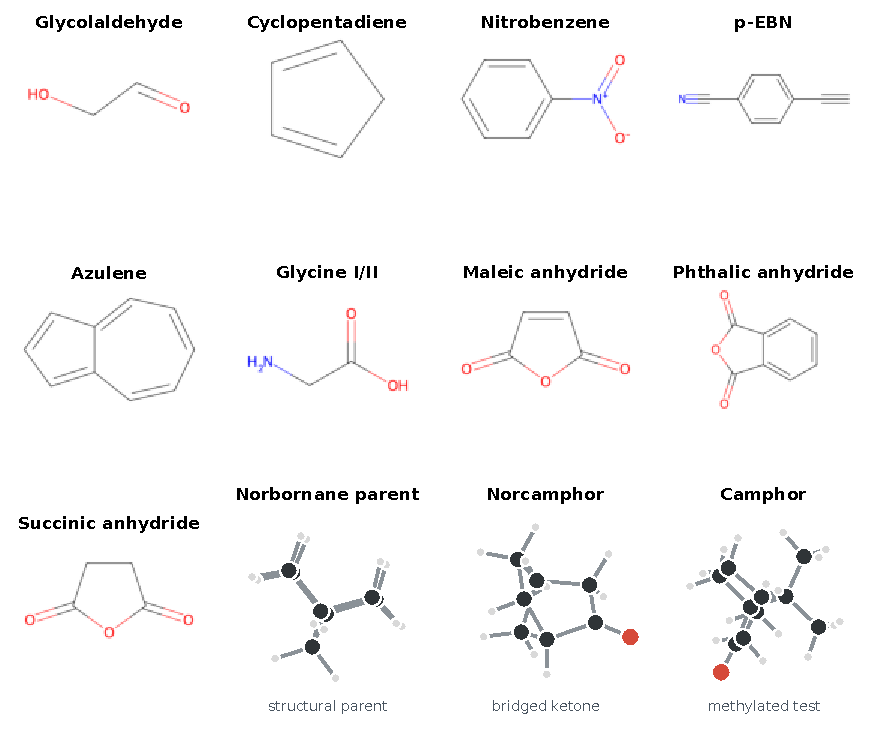
\includegraphics[width=0.96\linewidth]{figures/studied_structures_3d.pdf}
\caption{Molecular structures used to test automated model construction. The
acyclic, planar, aromatic, glycine, and anhydride benchmarks are shown as
connectivity diagrams; the bridged norbornane family is shown as
three-dimensional structures because its graph topology is not communicated
adequately by a planar drawing. Norbornane is included as the structural parent
of the bridged series, while norcamphor and camphor are the semiexperimental
validation cases. Testosterone is shown separately in the large-molecule scale
demonstration. Detailed atom numbering for the tabulated structural parameters
is given in the Supporting Information.}
\label{fig:studied-structures}
\end{figure*}

\begin{figure*}
\centering
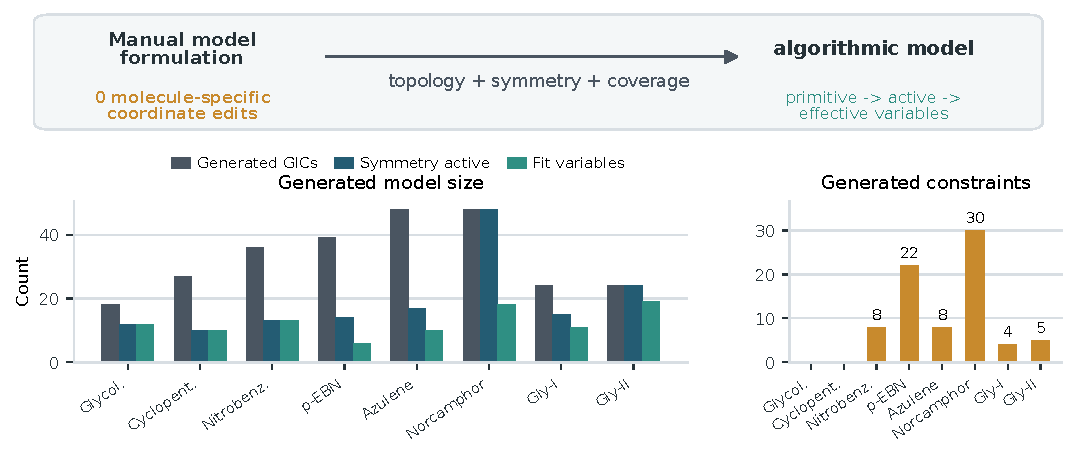
\includegraphics[width=0.92\linewidth]{figures/benchmark_overview.pdf}
\caption{Model-construction audit for the representative
refinements. The top guide links the manual formulation problem to the
generated model: topological analysis, symmetry assignment, and isotopic coverage
replace molecule-specific coordinate edits under the default global thresholds.
The left panel reports the number
of generated coordinates, the symmetry-active subset before
constraint projection, and the final least-squares variables after reduction.
The right panel reports the number of constraints or frozen primitive
parameters projected by the model layer. Manual coordinate-model edits are zero
for every case; global defaults can be inspected or overridden, but are not
tuned separately for the reported molecules. Detailed fit residuals and ranks are collected in the
Supporting Information.}
\label{fig:benchmark-overview}
\end{figure*}

Figure~\ref{fig:benchmark-overview} is the central validation of this logic:
it quantifies how topological analysis, symmetry assignment,
isotopic coverage, and reference information are transformed
into the final refinement model. The figure is therefore a
model-construction record, not simply a residual summary: it reports how many
primitive/non-redundant coordinates are produced, how many
remain active after symmetry selection, how many survive constraint
projection, and how many constraints are introduced without manual parameter
selection. The rotational residuals remain in the expected semiexperimental
range for standard, cyclic, planar, fused, bridged, and glycine benchmarks,
but the central result is that these residuals are obtained from generated,
reproducible models. The glycine examples also separate two roles of theory:
Gly-I starts from a reference that already satisfies the practical
rotational-accuracy target, whereas Gly-II uses QC-derived relations to define
missing reduced-dimensionality information. The numerical counterpart of this
graphical summary is given explicitly in the Supporting Information: the
working-coordinate table lists the generated models and active dimensions,
while the legacy-compatibility table shows that imported MSR/MSROT numerical
models are reproduced without changing their active-coordinate content.

Figure~\ref{fig:benchmark-overview} also makes explicit what is generated.
For azulene, topology and symmetry generate 48 final GICs, identify 17
totally symmetric coordinates, and reduce the fit to 10 effective variables
without a manual choice of refined coordinates. For norcamphor, the same
machinery constructs a non-redundant 48-coordinate GIC model for a
low-symmetry bridged system, then generates 30 hydrogen-frame constraints and
leaves 18 effective variables. These are the cases in which manual model
formulation is most exposed: fused rings and bridged frameworks make it
difficult to decide by inspection which distances, angles, torsions, and
hydrogen-frame quantities should be refined, tied, or constrained.
Table~\ref{tab:manual-vs-morpheus} recasts the same information as an
operator comparison. The comparison is not based on elapsed time, which is
operator- and implementation-dependent, but on reproducible decision classes:
which cyclic or bridged coordinates to use, which symmetry block to refine,
which unsupported directions require constraints, which planar rotational
components are admissible, and which parameters must remain active after rank
projection. In a manual workflow these choices precede the least-squares
solution and are a common source of non-reproducibility. In the reported runs
they are made by topological analysis, symmetry assignment, coverage analysis,
and rank checks. Thus the comparison is a test of reproducible model
formulation, not only of the numerical least-squares solution.

\begin{table*}
\caption{Decision burden removed by generated refinement models. Manual setup time
is not reported because it depends on operator choices; the table therefore
reports the reproducible decision burden. The final column counts
molecule-specific coordinate or constraint edits made by the user in the
reported runs.}
\label{tab:manual-vs-morpheus}
\scriptsize
\setlength{\tabcolsep}{1.5pt}
\begin{tabular*}{\textwidth}{@{\extracolsep{\fill}}lllll@{}}
\toprule
Case & Manual burden removed & Model & Constraints/classes & Outcome \\
\midrule
Azulene &
fused rings; symmetry; planar pair &
48 GICs; 17 sym.; 10 var. &
8 primitive constr. &
0.073 MHz RMS; 0 edits \\
Norcamphor &
bridged graph; H frames; covariance &
48 GICs; 48 active; 18 var. &
30 H-frame constr.; 58 predicates &
0.094 MHz RMS; 0 edits \\
Glycine I &
symmetry; unsupported H directions &
24 GICs; 15 $A'$; 11 var. &
4 QC constr. &
0.0269 MHz RMS; 0 edits \\
Glycine II &
low symmetry; coupled descriptors &
24 GICs; 19 var. &
5 QC constr.; classes &
0.249 MHz RMS; 0 edits \\
\bottomrule
\end{tabular*}
\end{table*}

The agreement with reference-quality refinements is therefore obtained after
removing the molecule-specific model-design step, not after tuning it.

The three anhydrides were selected as a homologous literature-data series
with a common chemical motif but progressively
different experimental completeness, and therefore test different parts of
the model layer. Maleic anhydride is the fully determined case: the published
work of Vogt, Demaison, and Rudolph\cite{Vogt2011MaleicAnhydride} reports the
parent geometry, ground-state rotational constants, rovibrational corrections,
and semiexperimental constants for a sufficiently rich isotopic set. Phthalic
anhydride tests mixed estimation: Belyakov et
al.\cite{Belyakov2022PhthalicAnhydride} supplement the rotational data with
weighted $r_e^\mathrm{BO}$ predicates. Succinic anhydride tests the opposite
limit: Jahn et al.\cite{Jahn2020SuccinicAnhydride} provide only heavy-atom
substitutions, so the hydrogen frame is not experimentally resolved and must be
represented by explicit model relations.

This series also makes the input claim concrete. Once $B_0$ constants and
rovibrational corrections $\Delta B_\mathrm{vib}$ are available, the
user transcribes the parent Cartesian geometry, the isotope
substitutions, and the tabulated corrections. The workflow then calls ORACLE
for perception and the primitive/B source, calls SMITH for the non-redundant
coordinate model, and lets the MORPHEUS model layer apply any necessary
constraints, predicates, or parameter classes as explicit statistical
relations.

For maleic anhydride no auxiliary relation is introduced and 21
non-redundant symmetry coordinates are generated, of which the eight $A_1$
coordinates are the active variables for the planar SE fit. The complete
symmetry-block inventory is reported in the Supporting Information.
The GIC and symmetry-Cartesian routes both give rank 8 and a rotational RMS
residual of 0.036~MHz; the recovered bond lengths agree with the published
$r_e^\mathrm{SE}$ values within $1.2\times10^{-4}$~\AA.

Table~\ref{tab:generated-relation-example} illustrates the type of chemically
meaningful relations generated by the advisor. The program
identifies unsupported structural directions and expresses them as primitive
internal-coordinate relations, which are subsequently projected onto the
algorithmically generated active space. The same representation also makes
ring coordinates explicit: endocyclic bends are generated from primitive
valence angles, while ring-puckering descriptors such as $q$ and $\phi$ are
derived from the cyclic U-based (RPck) block rather than selected as
molecule-specific torsions.

\begin{table*}[t]
\caption{Chemically readable primitive-coordinate relations generated by the
model layer. The first four entries are representative reduced-dimensionality
constraints for glycine; the last two show the corresponding form of generated
ring coordinates. Atom labels are used for readability.}
\label{tab:generated-relation-example}
\scriptsize
\setlength{\tabcolsep}{4pt}
\begin{tabular}{@{}lll@{}}
\toprule
Primitive relation & Generated relation & Role \\
\midrule
O--H bond & \texttt{ROH = R(O,H)} & fixes unsupported O--H distance \\
C--O--H angle & \texttt{AOH = A(C,O,H)} & preserves hydroxyl orientation \\
H--N--H angle & \texttt{HNH = A(H,N,H')} & constrains amino frame \\
NH$_2$ wag & \texttt{WNH2 = OOP(H,N,H',C)} & removes unsupported wagging direction \\
Endocyclic bend & \texttt{RB = sum c(i) A(i,j,k)} & defines ring valence coordinate \\
Ring puckering & \texttt{RPck = sum c(i) U(i); q, phi = f(RPck)} & U-based local puckering with derived global descriptors \\
\bottomrule
\end{tabular}
\end{table*}

For phthalic anhydride, the rotational information alone can give a small
rotational residual while leaving the structural model rank deficient. The
published solution is therefore naturally expressed as primitive-coordinate
predicates with conservative uncertainties of 0.002~\AA{} for bond lengths and
0.2$^\circ$ for angles. With these predicates, the fit has
rank 14, condition number 4.05, and a rotational RMS residual of 0.50~MHz. It
recovers the published $r_e^\mathrm{SE}$ structure within 0.0015~\AA{} for the
tabulated bond lengths and within 0.09$^\circ$ for the tabulated angles.

\begin{table*}[t]
\caption{Effect of auxiliary model relations for phthalic anhydride. The
predicate model uses the conservative $r_e^\mathrm{BO}$ uncertainties reported
by Belyakov et al. and the same literature rotational data. Structural errors are
maximum absolute deviations from the tabulated $r_e^\mathrm{SE}$ bond lengths or angles.}
\label{tab:phthalic-predicates}
\scriptsize
\setlength{\tabcolsep}{2.5pt}
\begin{tabular}{lcccc}
\toprule
Auxiliary relation & Rank & Cond. & RMS & Error \\
\midrule
None & 13 & $\infty$ & 0.0065 & 3.13$^\circ$ \\
Frozen H frames & 9 & 1056 & 0.0067 & 0.19$^\circ$ \\
$r_e^\mathrm{BO}$ predicates & 14 & 4.05 & 0.50 & 0.0015~\AA; 0.09$^\circ$ \\
\bottomrule
\end{tabular}
\end{table*}

Succinic anhydride completes the series because only heavy atoms are
isotopically substituted. The heavy-atom framework is determined, but the
hydrogen positions are not independent spectroscopic observables. In this case
a local hydrogen-frame constraint gives a stable fit with rank 5 and a
rotational RMS residual of 0.035~MHz. Weighted C--H predicates are still useful
diagnostically, but as soft observations they do not remove all unobserved
hydrogen-frame directions; without an additional topological or constraint
relation the optimizer can enter geometrically equivalent but chemically
unacceptable valleys. The comparison makes the distinction operational:
constraints remove unsupported directions, predicates add observations with
declared uncertainty, and parameter classes tie equivalent corrections.

\begin{figure}[!htb]
\centering
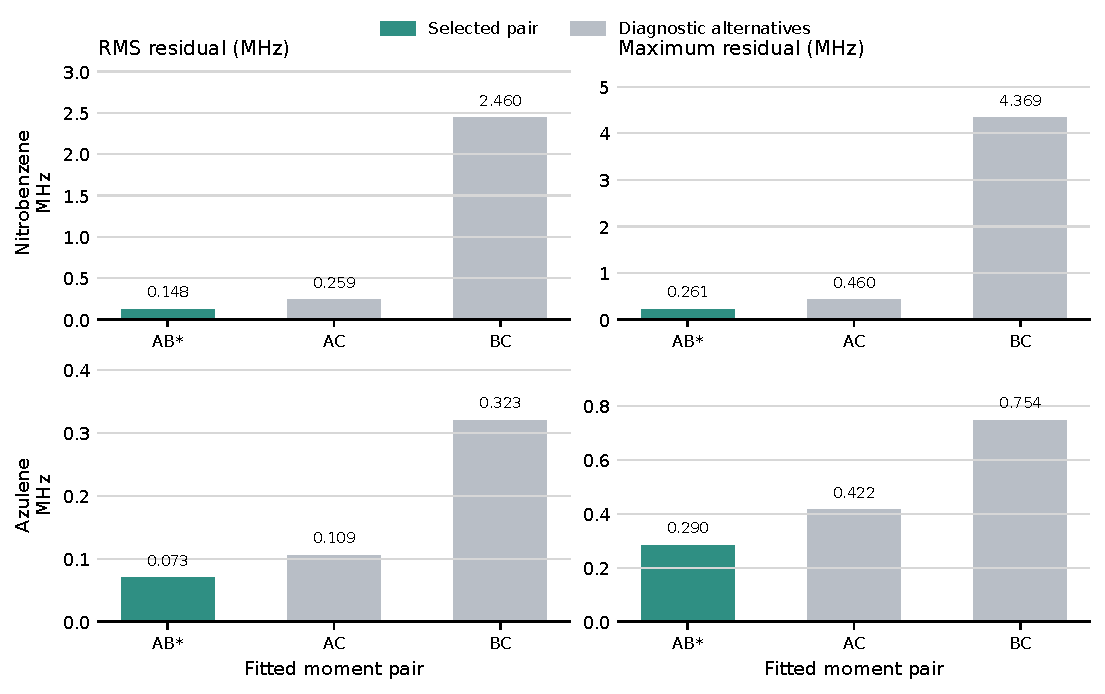
\includegraphics[width=0.82\linewidth]{figures/planar_pair_diagnostics.pdf}
\caption{Planar-component selection for nitrobenzene and azulene: the selected
$AB$ pair is highlighted and minimizes the complete post-fit diagnostic residual
while the omitted component remains
an external check. Detailed values are reported in the Supporting Information.}
\label{fig:planar-pair-diagnostics}
\end{figure}

For planar molecules the model layer selects the best pair of rotational
constants to be fitted, and retains the third rotational constant as
an external check computed from the final Cartesian geometry.
Figure~\ref{fig:planar-pair-diagnostics} shows that the $AB$ pair gives the
smallest complete diagnostic residual for both nitrobenzene and azulene.

The condition numbers in the benchmark table should be interpreted as
diagnostics of the inverse problem, not as residual-quality measures.
Nitrobenzene is the clearest example. It fits only the planar $AB$ component
pair from nine isotopologues while retaining 13 active variables and eight
primitive constraints; several deuterated substitutions therefore carry
substantial leverage on directions that are weakly separated by the moments of
inertia. The result is a high condition number
($2.75\times10^4$) even though the final rotational RMS residual is only
0.148~MHz. Azulene, by contrast, has a larger fused-ring coordinate space but
the algorithmic reduction leaves only 10 effective variables, and the
additional isotopic coverage and primitive constraints distribute the
spectroscopic information more evenly. Its condition number is therefore
lower ($9.57\times10^2$) despite the more complex topology. The same reading
applies to the other benchmarks: high condition numbers flag directions whose
uncertainties or influence diagnostics must be inspected, whereas acceptable
residuals alone do not prove that the structural model is statistically
well supported.

\begin{table}[t]
\caption{Leave-one-isotopologue sensitivity diagnostics for representative refinements. The table reports exact refits in which one isotopologue is omitted, followed by prediction of the omitted rotational constants.}
\label{tab:leave-one-out-sensitivity}
\scriptsize
\setlength{\tabcolsep}{3.0pt}
\resizebox{\columnwidth}{!}{%
\begin{tabular}{lrrrrr}
\toprule
System & Refits & Worst omitted RMS & Omitted & Max Cartesian shift & Cond. range \\
 & & MHz & & \AA & \\
\midrule
Maleic anhydride & 10 & 0.086 & 13C2d2 & 0.0005 & $6.1\times10^2$--$8.0\times10^2$ \\
Nitrobenzene & 9 & 0.388 & 3D & 0.0840 & $2.6\times10^4$--$3.7\times10^5$ \\
\bottomrule
\end{tabular}
}
\end{table}


Table~\ref{tab:leave-one-out-sensitivity} gives a direct sensitivity check.
Maleic anhydride is stable under exact leave-one-isotopologue refits: the
worst omitted-isotopologue RMS is 0.086~MHz and the largest Cartesian shift is
$5\times10^{-4}$~\AA. Nitrobenzene remains predictive for most omissions, but
the deuterated isotopologues expose the expected weak directions: the worst
omitted RMS rises to 0.388~MHz and one refit reaches a condition number of
$3.7\times10^5$. This is precisely the regime in which the algorithmic
model is useful to an operator: it does not hide the problem behind a small
training residual, but reports the rank, condition number, influence, and
leave-one-out diagnostics needed to decide whether additional data or stronger
model relations are required.

\begin{figure}
\centering
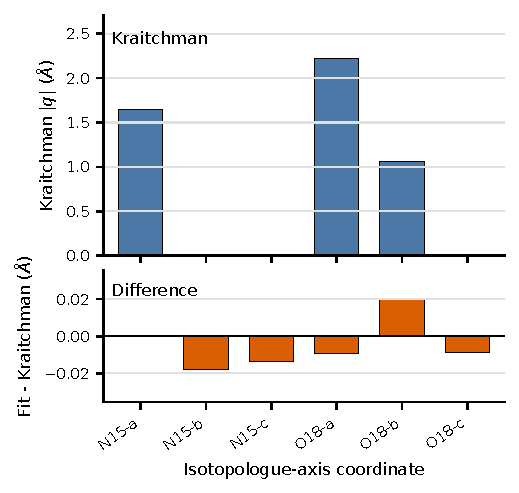
\includegraphics[width=0.92\linewidth]{figures/nitrobenzene_kraitchman_fit.pdf}
\caption{Kraitchman diagnostic for the nitrobenzene planar benchmark. The
upper panel reports absolute substitution coordinates from the Kraitchman
analysis. The lower panel reports signed differences between the final SE
coordinates and the Kraitchman values on an expanded scale. Numerical values
are reported in the Supporting Information.}
\label{fig:nitrobenzene-kraitchman-fit}
\end{figure}

The next two diagnostics compare the fitted structures with independent
structural information without changing the least-squares objective. The
nitrobenzene Kraitchman comparison in
Figure~\ref{fig:nitrobenzene-kraitchman-fit} confirms that the fitted
Cartesian structure follows the substitution-coordinate pattern, while the fit
itself remains based on moments of inertia. This is the intended use of
Kraitchman information here: it validates the SE+fit geometry but does not
replace the statistically coupled refinement.

\begin{figure*}
\centering
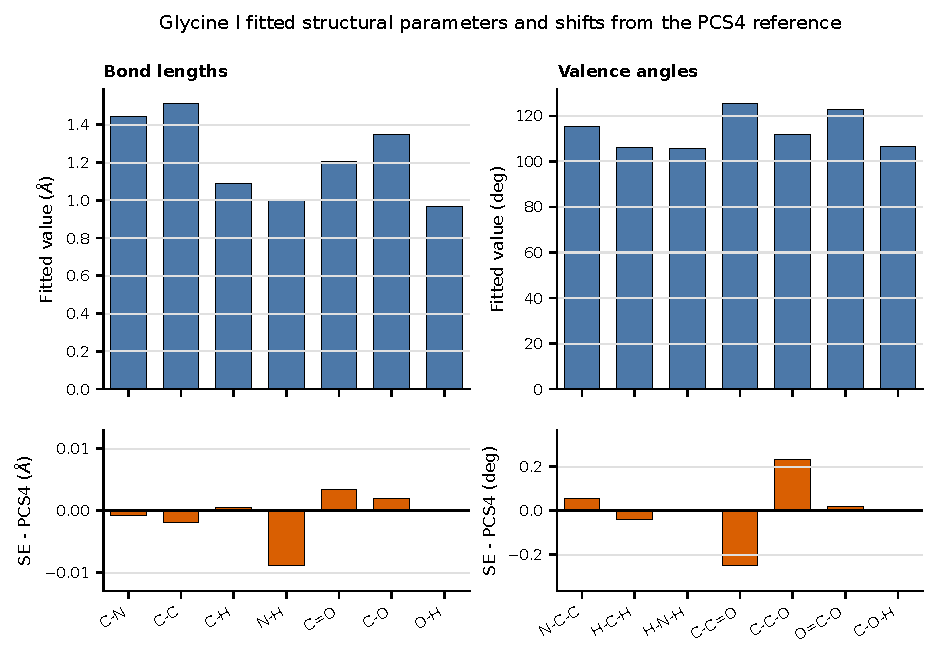
\includegraphics[width=0.94\linewidth]{figures/glycine_I_qc_fit_parameters.pdf}
\caption{Glycine I fitted structural parameters and shifts from the QC
reference geometry. The upper panels report final SE bond lengths and
valence angles; the lower panels report signed SE--QC differences on
expanded scales.}
\label{fig:glycine-I-qc-parameters}
\end{figure*}

The Gly-I structural comparison in
Figure~\ref{fig:glycine-I-qc-parameters} shows the scale of the
semiexperimental correction when the starting QC geometry already reproduces
the rotational data well. Since the reduced-dimensionality constraints are
generated from the QC reference structure, the small SE--QC differences
provide an a posteriori validation of the generated constraint
model, not merely a check that the starting geometry was good.

Detailed atom numbering, rotational constants, topological parameters,
Kraitchman diagnostics, reference-geometry comparisons, residuals, conditioning, and
covariance diagnostics are reported in the Supporting Information. The main text
retains the information needed to
assess model formulation: rank, dimensionality, symmetry, constraint
projection, planar-component choice, residual scale, and minimum checks.

\subsection{Generated Reduced-Dimensionality and Validation Models}

Incomplete isotopic coverage can leave some structural directions unsupported.
The advisor therefore treats reduced dimensionality as part of the
model-generation step. It preserves the highest compatible symmetry, identifies
local coordinates that cannot be determined independently, and replaces them
by primitive-coordinate constraints, predicates, or parameter classes.

\begin{table*}
\caption{Autonomous structural-model decisions made by the advisor in the
reduced-dimensionality and validation benchmarks. ``Active variables'' are the
independent least-squares coordinates after symmetry selection and projection
of hard primitive-coordinate constraints.}
\label{tab:advisor-decisions}
\small
\setlength{\tabcolsep}{3.5pt}
\begin{tabular}{@{}lllll@{}}
\toprule
System & GIC space & Variables & Generated constraints & Classes \\
\midrule
Glycine I & 24 GICs; 15 $A'$ & 11 & 4 QC constraints & none \\
Glycine II & 24 GICs; C$_1$ & 19 & 5 QC constraints & coupled descriptors \\
Norcamphor & 48 GICs; C$_1$ & 18 & 30 H-frame; 58 Kraitchman & constrained H frames \\
Camphor & 75 GICs; C$_1$ & 75 & 178 BDPCS3 predicates; no Kraitchman & validation-controlled predicates \\
\bottomrule
\end{tabular}
\end{table*}

Table~\ref{tab:advisor-decisions} shows that the reduced models are generated
from isotope coverage and chemical equivalence rather than imported as a
manual parameter subset. In glycine I, glycine II, and norcamphor the available
substitutions do not support all hydrogen-related directions independently;
the advisor therefore converts the unsupported directions into explicit
primitive-coordinate relations derived from the reference structure.

The bridged cases are best viewed as a norbornane-derived progression.
Norbornane defines the bicyclic topology, norcamphor adds the ketone and
sparse heavy-atom substitution data, and camphor adds methyl substitution and
a larger set of local hydrogen directions. Norcamphor is therefore the
reduced-dimensionality member of the series: all 48 GICs belong to the
totally symmetric space, so the reduction is controlled by coverage and
local-frame diagnostics rather than by point-group symmetry. The updated
\texttt{xyzin} input uses the experimental constants of Table 3 of the
norcamphor rotational study, the tabulated vibrational corrections, and
Kraitchman-derived soft predicates generated from the singly substituted
heavy-atom isotopologues. The workflow uses 30 hydrogen-frame constraints and
58 \mbox{Kraitchman predicates} to obtain an 18-dimensional fit with a
rotational RMS residual of 0.094~MHz.

Camphor then tests the complementary question: not whether unsupported
directions can be stabilized, but whether a generated model can reject a
tempting but chemically wrong stabilization in the same bridged family. The
accepted run uses 12 isotopologue records, 36 rotational constants, a
full-rank 75-variable GIC model, and 178 BDPCS3 soft predicates; no hydrogen
coordinate is frozen and no Kraitchman-derived predicate is retained in the
least-squares objective. The rotational RMS residual is 0.0788~MHz, with a
maximum absolute residual of 0.284~MHz. More importantly, the final structural
correction to the BDPCS3 reference remains small on the chemically relevant
scale: the largest bond-length shift is 0.832~m\AA{}, the largest
valence-angle shift is $0.040^\circ$, and the corresponding propagated
standard errors are bounded by 3.000~m\AA{} and $0.257^\circ$.

Camphor is deliberately used as the full validation stress test because it is
the exposed full-rank member of the bridged series: the model retains all 75
GIC variables and is stabilized by soft predicates rather than by removing
unsupported directions through hard constraints. The reduced-dimensionality
benchmarks require rank, covariance, and leave-one-isotopologue checks, but
they do not require the same exhaustive predicate-width and leave-group-out
campaign because their unsupported directions have already been projected out
of the fit.

The validation suite makes this distinction quantitative. Replaying the same
model in the symmetry-adapted Cartesian basis changes the aligned Cartesian
structure by only $5.2\times 10^{-11}$~\AA{} RMS; robust-loss and multistart
checks change it by less than $5\times10^{-4}$~\AA{} RMS, and predicate-width
scans keep the maximum atomic displacement below $9.5\times10^{-4}$~\AA{}.
By contrast, removing hydrogen-related predicates gives lower or comparable
rotational residuals but shifts atoms by up to 0.935~\AA{}, and tight
Kraitchman predicates produce bond and angle distortions up to 7.65~m\AA{}
and $0.343^\circ$. Broad Kraitchman predicates are not damaging, but they do
not add useful information to the validated BDPCS3-predicate model. The
camphor member of the bridged series therefore shows the operational role of
the advisor: it does not merely assemble a least-squares input, it proposes a
chemically explicit model and then rejects variants that fail reproducibility,
robustness, or structural-stability checks.

\begin{widetext}
\begin{center}
\refstepcounter{table}
\label{tab:camphor-final-validation}
\parbox{0.96\textwidth}{\small\raggedright Table~\thetable: Camphor
final-validation controls. RMSD and maximum atomic shifts are computed after
alignment to the accepted no-Kraitchman BDPCS3-predicate reference geometry.\par}
\smallskip
\footnotesize
\setlength{\tabcolsep}{4pt}
\begin{tabular}{lrrrrl}
\toprule
Check & Runs & Max RMS/MHz & Max RMSD/\AA{} & Max atom/\AA{} & Interpretation \\
\midrule
Coordinate-model replay & 1 & 0.0788 & $5.24\times10^{-11}$ & $1.12\times10^{-10}$ & basis independent \\
Huber robust loss & 1 & 0.1388 & $1.93\times10^{-4}$ & $3.67\times10^{-4}$ & stable \\
Predicate sigma scans & 12 & 0.0868 & $3.56\times10^{-4}$ & $9.48\times10^{-4}$ & stable \\
Random multistarts & 5 & 0.0788 & $4.74\times10^{-4}$ & $6.92\times10^{-4}$ & stable \\
Leave non-H predicate groups out & 3 & 0.0778 & 0.0040 & 0.0137 & moderate drift \\
Leave H predicate groups out & 3 & 0.0777 & 0.3039 & 0.9347 & failure mode \\
\bottomrule
\end{tabular}
\end{center}
\end{widetext}

Table~\ref{tab:camphor-final-validation} summarizes the corresponding
coordinate-basis replay, robust loss, predicate-width scans, multistarts, and
leave-predicate-group-out controls.

\begin{figure*}[t]
\centering
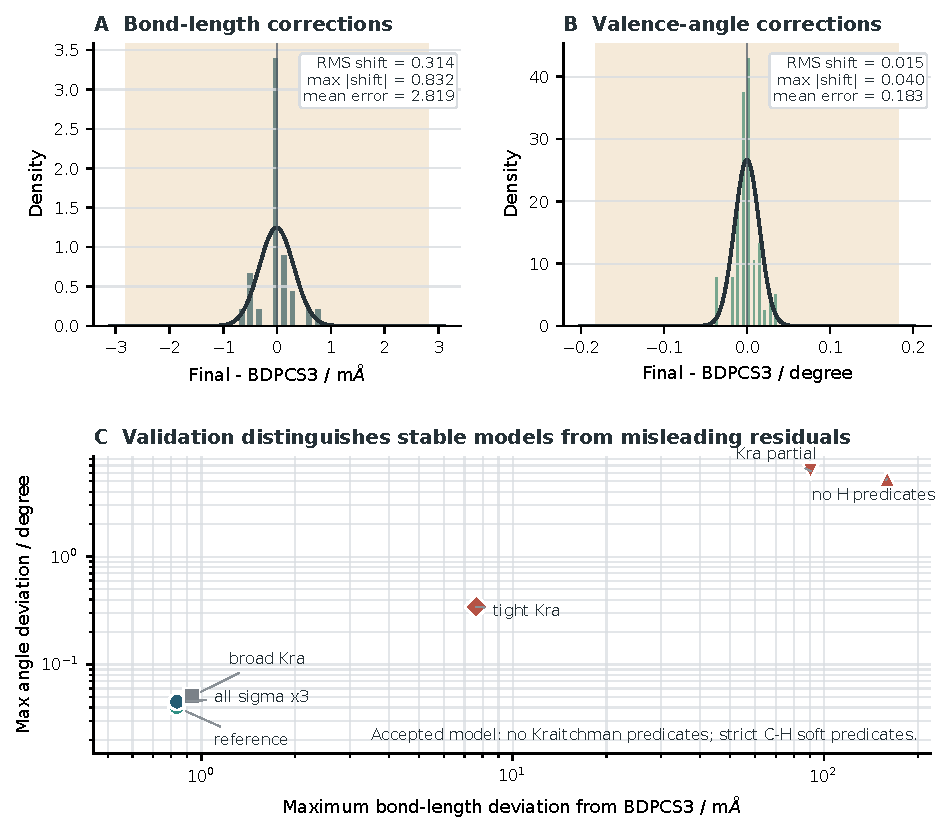
\includegraphics[width=0.92\linewidth]{figures/camphor_validation_distributions.pdf}
\caption{Camphor validation stress test. Panels A and B show the signed
final-minus-BDPCS3 shifts for bond lengths and valence angles in the accepted
no-Kraitchman model; the curves are normal distributions fitted to the signed
shifts, and the shaded intervals indicate the mean propagated standard error.
Panel C compares selected stability variants by the maximum structural
deviation from the BDPCS3 reference. The accepted model and predicate-width
perturbations remain in the sub-milliangstrom, few-hundredths-of-a-degree
region, whereas models that remove hydrogen predicates or impose tight
Kraitchman-derived predicates can yield superficially acceptable rotational
residuals while distorting the geometry.}
\label{fig:camphor-validation}
\end{figure*}

\subsection{Glycine as an End-to-End Model-Generation Test}

The two glycine conformers test the same model-generation layer starting
from QC geometries when hydrogen-related directions are only partly supported.

\begin{figure*}
\centering
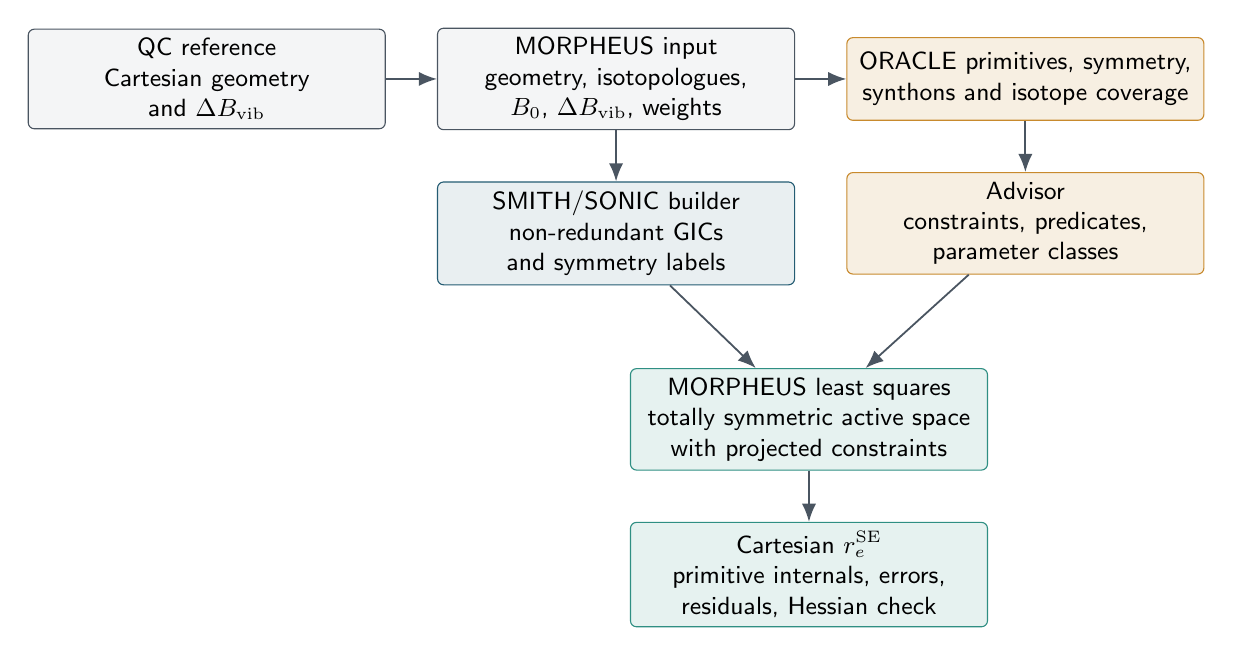
\begin{tikzpicture}[
  node distance=0.65cm,
  stepbox/.style={
    draw=FrameworkSlate,
    fill=FrameworkSlate!6,
    rounded corners=2.2pt,
    align=center,
    text width=4.3cm,
    minimum height=1.05cm,
    font=\small\sffamily
  },
  autobox/.style={stepbox, draw=FrameworkBlue, fill=FrameworkBlue!10},
  chemobox/.style={stepbox, draw=FrameworkGold, fill=FrameworkGold!14},
  fitbox/.style={stepbox, draw=FrameworkTeal, fill=FrameworkTeal!12},
  flowarrow/.style={-{Latex[length=2.3mm,width=1.8mm]}, line width=0.65pt, draw=FrameworkSlate}
]
\node[stepbox] (pcs) {QC reference\\Cartesian geometry\\and $\Delta B_\mathrm{vib}$};
\node[stepbox, right=0.65cm of pcs] (job) {MORPHEUS input\\geometry, isotopologues,\\$B_0$, $\Delta B_\mathrm{vib}$, weights};
\node[chemobox, right=0.65cm of job] (syn) {ORACLE primitives, symmetry,\\synthons and isotope coverage};
\node[chemobox, below=0.65cm of syn] (adv) {Advisor\\constraints, predicates,\\parameter classes};
\node[autobox, below=0.65cm of job] (gic) {SMITH/SONIC builder\\non-redundant GICs\\and symmetry labels};
\node[fitbox, below=1.05cm of gic, xshift=2.45cm] (fit) {MORPHEUS least squares\\totally symmetric active space\\with projected constraints};
\node[fitbox, below=0.65cm of fit] (out) {Cartesian $r_e^\mathrm{SE}$\\primitive internals, errors,\\residuals, Hessian check};
\draw[flowarrow] (pcs) -- (job);
\draw[flowarrow] (job) -- (syn);
\draw[flowarrow] (syn) -- (adv);
\draw[flowarrow] (job) -- (gic);
\draw[flowarrow] (gic) -- (fit);
\draw[flowarrow] (adv) -- (fit);
\draw[flowarrow] (fit) -- (out);
\end{tikzpicture}
\caption{End-to-end glycine refinement starting from QC Cartesian reference
geometries and vibrational corrections.
The calculation uses the common job/xyzin container, chemical descriptors, and isotope
coverage to generate the active coordinate and constraint model without manually
selected fit variables.}
\label{fig:glycine-algorithmic-flow}
\end{figure*}

For glycine I, the parent, $^{13}$C(carboxyl), $^{13}$C(methylene), CD$_2$,
and $^{15}$N isotopologues are fitted using the rotational constants and
weights of Godfrey and Brown\cite{GodfreyBrown1995ShapeGlycine} and the
zero-point corrections of Kasalov{\'a} et al.\cite{Kasalova2007Glycine} The
QC reference already reproduces the 15 vibrationally corrected constants
with an RMS relative error of 0.0258\% and a maximum error of 0.0363\%. The
advisor detects the C$_s$ geometry and incomplete hydrogen information and
generates four constraints: O--H distance, C--O--H angle, H--N--H angle, and
NH$_2$ wag. Projection leaves 11 independent variables from 15 $A'$ GICs, and
the final fit gives a complete rotational RMS residual of 0.0269 MHz with a
positive optimized-space Hessian.

% Generated from the glycine I QC-reference semiexperimental run.
\begin{table}
\caption{Glycine I rotational residuals for the quantum-chemical reference and
final semiexperimental geometries over five isotopologues.}
\label{tab:glycine-I-qc-rotational}
\scriptsize
\setlength{\tabcolsep}{3pt}
\begin{tabular}{lrrrr}
\toprule
Geometry & RMS/MHz & Max/MHz & RMS/\% & Max/\% \\
\midrule
QC reference & 1.7414 & 3.4072 & 0.0258 & 0.0363 \\
SE fit & 0.0269 & 0.0571 & 0.0005 & 0.0011 \\
\bottomrule
\end{tabular}
\end{table}

\begin{table}
\caption{Parent glycine I rotational constants from the quantum-chemical
reference and final semiexperimental geometries, in MHz.}
\label{tab:glycine-I-parent-rotational}
\scriptsize
\setlength{\tabcolsep}{2pt}
\begin{tabular}{lrrrrr}
\toprule
Component & Exp. $B_e$ & QC & QC--Exp. & SE & SE--Exp. \\
\midrule
A & 10420.1910 & 10422.9024 & 2.7114 & 10420.2481 & 0.0571 \\
B & 3907.4785 & 3907.5931 & 0.1146 & 3907.4786 & 0.0001 \\
C & 2934.6809 & 2935.7175 & 1.0366 & 2934.6808 & -0.0001 \\
\bottomrule
\end{tabular}
\end{table}


The same Gly-I model was also rerun with weighted initial-geometry predicates
on XY and X--H distances and selected heavy-atom/C--O--H angles
($\sigma_R=0.003$~\AA{}, $\sigma_A=0.3^\circ$). The rank remains 11, the
condition number decreases from $1.02\times10^4$ to $8.02\times10^3$, and the
complete rotational RMS changes only from 0.0269 to 0.0389 MHz. The propagated
uncertainties remain chemically meaningful: the largest reported bond-length
uncertainty is 0.0017~\AA{} and the largest valence-angle uncertainty is
0.12$^\circ$. Thus, for a high-quality PCS4 starting geometry, predicates act
as a conservative stabilization layer rather than as hidden constraints.

The Gly-I comparison is intentionally stringent: the refinement starts from an
already spectroscopically consistent QC structure rather than correcting a poor
starting point. The largest heavy-atom bond and valence-angle shifts relative
to the final semiexperimental structure are 0.0034~\AA\ and 0.25$^\circ$,
respectively, both within the scale expected for state-of-the-art QC structures
and vibrational corrections.\cite{PuzzariniStanton2023,Mendolicchio2025FastDvib}

Glycine II is the non-symmetric reduced-dimensionality case. The available
isotopologues do not determine a stable full structure, so the QC reference
is used to generate coupled primitive-coordinate constraints: C--H and N--H
differences, two methylene angular combinations, and an average H--N--C--C
torsion. These constraints are then projected onto the
24-dimensional C$_1$ GIC space.

\begin{center}
\refstepcounter{table}
\label{tab:glycine-constraint-comparison}
\parbox{0.94\linewidth}{\small\raggedright Table~\thetable: Glycine II
constraint-source comparison. Both calculations used GIC coordinates, moments
of inertia as observables, and the same 10 corrected Gly-IIn rotational data
sets. Rotational residuals are reported over the diagnostic $A$, $B$, and $C$
constants in MHz. The last column is the mean-square convention used for
comparison with the published glycine refinement, not a second RMS value.\par}
\smallskip
\small
\begin{tabular}{lrrrr}
\toprule
Constraint target source & Rank & RMS & Max & $10^3\langle\Delta B^2\rangle$ \\
\midrule
Kasalov{\'a}-type values & 19 & 0.2344 & 0.8100 & 54.94 \\
QC-derived values & 19 & 0.2491 & 0.6707 & 62.06 \\
\bottomrule
\end{tabular}
\end{center}

Table~\ref{tab:glycine-constraint-comparison} shows that QC-derived targets
produce the same rank and essentially the same residual scale as the published
Kasalov{\'a}-type constraints. The final QC-constrained refinement has 19
effective variables, a condition number of $1.05\times10^4$, and a complete
rotational RMS residual of 0.2491 MHz. The largest uncertainties remain in the
amino-hydrogen frame, as expected from the substitution pattern.

Adding the same weighted predicate layer to the QC-constrained Gly-II model
preserves the rank at 19, lowers the condition number to $8.55\times10^3$, and
gives a complete rotational RMS of 0.2401 MHz. The heavy-atom bond
uncertainties remain below 0.0024~\AA{} and the heavy-atom valence-angle
uncertainties below 0.25$^\circ$, whereas several amino-hydrogen angles and
torsions retain larger propagated uncertainties. MORPHEUS therefore reports
the predicates as useful stabilization and diagnostics, but does not interpret
the poorly substituted hydrogen-frame directions as fully determined structural
parameters.

\begin{center}
\refstepcounter{table}
\label{tab:glycine-predicate-checks}
\parbox{0.94\linewidth}{\small\raggedright Table~\thetable: Effect of weighted
predicates on the glycine reduced-dimensionality fits. The predicate runs use
the same experimental data and hard functional constraints as the corresponding
benchmark runs, plus initial-geometry predicates with $\sigma_R=0.003$~\AA{},
$\sigma_A=0.3^\circ$, and $\sigma_D=0.5^\circ$. RMS values are complete
rotational residuals in MHz.\par}
\smallskip
\small
\setlength{\tabcolsep}{3pt}
\begin{tabular}{lrrr}
\toprule
Model & Rank & Cond. & RMS \\
\midrule
Gly-I constraints & 11 & $1.02\times10^4$ & 0.0269 \\
Gly-I + predicates & 11 & $8.02\times10^3$ & 0.0389 \\
Gly-II QC constraints & 19 & $1.05\times10^4$ & 0.2491 \\
Gly-II + predicates & 19 & $8.55\times10^3$ & 0.2401 \\
\bottomrule
\end{tabular}
\end{center}

\subsection{Testosterone: Large-Molecule Scale Demonstration}

The validation benchmarks above were selected because they represent available
experimental gold standards while spanning acyclic, cyclic, fused, bridged,
planar, homologous, and reduced-dimensionality cases. The model-generation
layer is not limited to these sizes. As a scale check, the framework was
also applied to testosterone, using the published experimental ground-state
rotational constants and vibrational corrections for the observed
T1-H2$^{-}$-gp conformer.\cite{Uribe2024SteroidHormones} This is a useful large
molecule test because this level of treatment is rarely available for systems
of this size: an accurate QC equilibrium geometry, accelerated
$\Delta B_\mathrm{vib}$ corrections, and automated model construction are
combined in one reproducible protocol.

The unrefined QC+$\Delta B_\mathrm{vib}$ residuals with respect to the corrected
experimental constants are $4.638$, $0.674$, and $0.563$ MHz for $A$, $B$, and
$C$, respectively. After a 141-dimensional non-redundant space is built, the
class layer applies a single graph-derived C--C skeletal stretch class.
Operationally, non-skeletal stretch combinations and the angular, torsional,
and out-of-plane families are held fixed for this parent-only diagnostic, while
the retained C--C stretch block is replaced by one shared variable after rank
reduction. The resulting refinement improves the residuals to $-0.027$,
$0.633$, and $0.292$ MHz, reducing the RMS rotational residual from 2.73 to
0.40 MHz. Two additional end-to-end variants test more informative model
formulations without changing the input data. Separating C--C and C--O stretch
classes gives residuals of $0.002$, $0.046$, and $-0.058$ MHz. In this run the
model is specified only through primitive C--C and C--O bond classes; MORPHEUS
maps the generated GICs onto disjoint shared classes with default coefficient
thresholds and an automatic data-compatible class budget, freezing unsupported
directions.
A predicate model that keeps a compact C--C/C--O subset independent and
constrains the corresponding XY QC bond lengths with 0.005~\AA{} uncertainties
gives $4.128$, $0.704$, and $0.555$ MHz. Relaxing the same XY predicates to
0.01~\AA{} improves these residuals to $3.114$, $0.755$, and $0.531$ MHz, but
still does not approach the two-class C--C/C--O result. Predicate widths should
reflect the expected accuracy of the QM reference: for a good equilibrium
geometry, 0.005--0.01~\AA{} is already a conservative XY-bond range, whereas
0.05~\AA{} would correspond to an unrealistically loose structural prior. The
test therefore shows that one parent isotopologue is too little information for
independent predicate-guided C--C/C--O corrections, and that the class model is
the appropriate reduced description in this limiting case. With several
isotopologues, even when the data set remains incomplete, the glycine tests show
that classes and predicates can be combined more effectively.
This test is deliberately not presented as an isotope-rich
structural validation: it demonstrates that a large-molecule QC geometry,
vibrational corrections, non-redundant coordinate generation, class constraints,
and weighted predicates can be chained for a 49-atom fused-ring molecule, where
sufficiently rich isotopic substitution data are not presently available for a
full validation of the fit engine.

\begin{center}
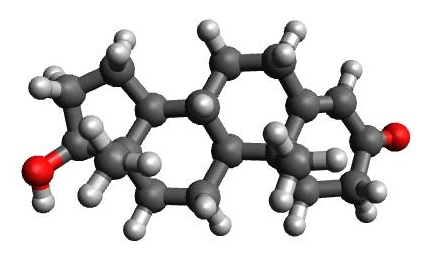
\includegraphics[width=0.90\linewidth]{figures/testosterone_qc_cropped.jpg}

\smallskip
\footnotesize Testosterone large-molecule scale demonstration.

\medskip
\footnotesize
Residuals are relative to the corrected experimental equilibrium constants
derived from the published $B_0$ and $\Delta B_\mathrm{vib}$ values.

\smallskip
\begin{tabular}{lrrrr}
\toprule
Model & Variables & $\Delta A$ & $\Delta B$ & $\Delta C$ \\
\midrule
QC+$\Delta B_\mathrm{vib}$ & 0 & 4.638 & 0.674 & 0.563 \\
C--C class & 1 & -0.027 & 0.633 & 0.292 \\
C--C/C--O classes & 2 & 0.002 & 0.046 & -0.058 \\
XY QC predicates, 0.005~\AA{} & 7 & 4.128 & 0.704 & 0.555 \\
XY QC predicates, 0.01~\AA{} & 7 & 3.114 & 0.755 & 0.531 \\
\bottomrule
\end{tabular}
\end{center}

\section{Conclusions}

The central contribution of this work is a general framework for proposing and
validating constrained refinement models, demonstrated here through
semiexperimental structure refinement. Existing refinement methods generally
assume that the coordinate model has already been supplied; here topology
analysis, symmetry assignment, homogeneous rank pruning, constraint
projection, least-squares solution, covariance propagation, and final
model-stability checks are part of one calculation rather than separate user
decisions.

The benchmarks show that the resulting models remain topology-derived,
symmetry-consistent, rank-consistent, and non-redundant for acyclic, cyclic,
planar, fused, bridged, homologous anhydride, glycine, and large fused-ring
cases. The program selects the active symmetry space, removes redundant
coordinates, chooses the independent moment components for planar molecules,
generates constraints when isotopic coverage is incomplete, and propagates
covariance to the reported structural parameters. Where both active coordinate
models are applicable, GIC and symmetry-Cartesian refinements give the same
effective dimensions and rotational residuals.

Electronic-structure information is used only where the experiment does not
fully determine the structure. For Gly-I the QC reference already lies within
the practical rotational-accuracy window, so the fit provides a statistically
consistent semiexperimental correction and uncertainty estimate. For Gly-II
and norcamphor, the advisor converts reference information and isotope
coverage into explicit reduced-dimensionality constraints. The reference
therefore supplies constraints for unsupported directions, while the
spectroscopic data determine all supported directions.

The norbornane-derived series adds the decisive validation step. Norcamphor
shows that a bridged low-symmetry topology can be reduced to a stable
semiexperimental model when isotope coverage is incomplete. Camphor keeps the
same structural motif but adds methyl substitution and a denser set of
hydrogen-sensitive local directions. In that harder case, a model with strict
BDPCS3-derived C--H predicates and no Kraitchman predicates gives a
sub-milliangstrom correction to the reference geometry and remains stable
under coordinate-basis changes, robust losses, predicate-width scans, and
multistarts. Alternative models that look numerically attractive from the
rotational residual alone fail chemically when hydrogen predicates are removed
or Kraitchman-derived restraints are made too tight. This is the practical
reason for making model construction explicit: the residual is necessary, but
it is not a sufficient certificate of a meaningful structure.

This is not simply a convenient input generator. The final outputs remain
ordinary chemical objects: Cartesian structures, bond lengths, valence angles,
dihedrals, ring descriptors, propagated uncertainties, residuals, and
diagnostics. What changes is that the path from topology and data to those
objects is explicit, reproducible, rank-tested, and challenged by independent
stability checks, even for molecular graphs in which manual coordinate
formulation is often the limiting step.

The testosterone scale check extends this logic to the current upper end of
practical rotational-spectroscopic modeling. It does not claim a complete
semiexperimental structure from a parent-only data set; instead, it shows that
an accurate large-molecule QC geometry, accelerated $\Delta B_\mathrm{vib}$
corrections, algorithmic non-redundant GIC generation, and class-constrained
refinement can be chained for a 49-atom fused-ring molecule in a
reproducible calculation. This closes the loop from accurate
large-molecule QC structures to generated spectroscopic
refinement models.

The essential shift is from expert-dependent model formulation to reproducible
model generation integrated with the refinement itself. The
algorithm records and enforces chemical judgement in an explicit form rather
than replacing it with hidden manual choices. Although motivated by
semiexperimental equilibrium structures, the underlying graph-driven strategy
is applicable to any constrained refinement problem requiring simultaneous
treatment of topology, symmetry, rank deficiency, and external structural
information.

The Supporting Information is organized in three parts: benchmark diagnostics
and reproducibility; detailed validation studies for camphor, glycine, and the
anhydride series; and large-molecule scalability with complete archived
examples.

\section*{Supporting Information Available}

Atom-numbered structures for the benchmark and companion systems; complete
rotational-constant comparisons for glycine I, glycine II, cyclopentadiene,
nitrobenzene, and azulene; Kraitchman, reference-fit, and planar-component
diagnostics; additional diagnostic tables for glycolaldehyde, norcamphor, and
camphor; final Cartesian coordinates, propagated topological parameters,
residuals, and archived \texttt{MORPHEUS} output files.

\section*{Code Availability}

The benchmark input/output files, numerical audit trails, and statistical
diagnostics are documented in the Supporting Information. The code implementing
the least-squares refinement engine, job/\texttt{xyzin} readers, coordinate
contracts, and final-validation audit used for the benchmarks reported here is
available from the author upon request. The intramolecular primitive
definitions and Wilson $\mathbf{B}$ source used in the present work were
generated by \texttt{ORACLE}; their non-redundant transformations were stored
as \texttt{SONIC} contracts by \texttt{SMITH}. The companion
\texttt{SMITH}/\texttt{SONIC} methodological manuscript is available as a
companion work and can be supplied as confidential supplementary material for
referees if required by the journal. This does not affect the present
applications, because the final-validation workflow replays accepted models in
both the generated GIC basis and the independent symmetry-adapted Cartesian
basis whenever both representations are applicable.


\bibliographystyle{aipnum4-2}
\bibliography{references}

\end{document}
